% THIS IS SIGPROC-SP.TEX - VERSION 3.1
% WORKS WITH V3.2SP OF ACM_PROC_ARTICLE-SP.CLS
% APRIL 2009
%
% It is an example file showing how to use the 'acm_proc_article-sp.cls' V3.2SP
% LaTeX2e document class file for Conference Proceedings submissions.
% ----------------------------------------------------------------------------------------------------------------
% This .tex file (and associated .cls V3.2SP) *DOES NOT* produce:
%       1) The Permission Statement
%       2) The Conference (location) Info information
%       3) The Copyright Line with ACM data
%       4) Page numbering
% ---------------------------------------------------------------------------------------------------------------
% It is an example which *does* use the .bib file (from which the .bbl file
% is produced).
% REMEMBER HOWEVER: After having produced the .bbl file,
% and prior to final submission,
% you need to 'insert'  your .bbl file into your source .tex file so as to provide
% ONE 'self-contained' source file.
%
% Questions regarding SIGS should be sent to
% Adrienne Griscti ---> griscti@acm.org
%
% Questions/suggestions regarding the guidelines, .tex and .cls files, etc. to
% Gerald Murray ---> murray@hq.acm.org
%
% For tracking purposes - this is V3.1SP - APRIL 2009

\documentclass{acm_proc_article-sp}

\begin{document}

\title{Ramp it up! \\Action based guide for creating accessible websites\titlenote{The large format version of this poster is available at the author's website at \texttt{terracoda.net}}}
%
% You need the command \numberofauthors to handle the 'placement
% and alignment' of the authors beneath the title.
%
% For aesthetic reasons, we recommend 'three authors at a time'
% i.e. three 'name/affiliation blocks' be placed beneath the title.
%
% NOTE: You are NOT restricted in how many 'rows' of
% "name/affiliations" may appear. We just ask that you restrict
% the number of 'columns' to three.
%
% Because of the available 'opening page real-estate'
% we ask you to refrain from putting more than six authors
% (two rows with three columns) beneath the article title.
% More than six makes the first-page appear very cluttered indeed.
%
% Use the \alignauthor commands to handle the names
% and affiliations for an 'aesthetic maximum' of six authors.
% Add names, affiliations, addresses for
% the seventh etc. author(s) as the argument for the
% \additionalauthors command.
% These 'additional authors' will be output/set for you
% without further effort on your part as the last section in
% the body of your article BEFORE References or any Appendices.

\numberofauthors{1} %  in this sample file, there are a *total*
% of EIGHT authors. SIX appear on the 'first-page' (for formatting
% reasons) and the remaining two appear in the \additionalauthors section.
%
\author{
% You can go ahead and credit any number of authors here,
% e.g. one 'row of three' or two rows (consisting of one row of three
% and a second row of one, two or three).
%
% The command \alignauthor (no curly braces needed) should
% precede each author name, affiliation/snail-mail address and
% e-mail address. Additionally, tag each line of
% affiliation/address with \affaddr, and tag the
% e-mail address with \email.
%
% 1st. author
\alignauthor
Taliesin L. Smith\titlenote{The author is an MDes.(Candidate) Inclusive Design at OCAD University}\\
	   %\affaddr{Instructional Design Specialist}\\
       \affaddr{Memorial University}\\
       \affaddr{St. John's, Newfoundland Labrador, Canada}\\
       \email{tlsmith@mun.ca}
% 2nd. author
%\alignauthor
%T.L. Smith\titlenote{The secretary disavows
%any knowledge of this author's actions.}\\
%       \affaddr{OCAD University}\\
%       \affaddr{P.O. Box 1212}\\
%       \affaddr{Dublin, Ohio 43017-6221}\\
%       \email{webmaster@marysville-ohio.com}
}
\date{10 January 2015}

\maketitle
\begin{abstract}
\textit{Ramp it up} is an action based guide for coding in the virtual ramp to make websites and website content accessible to people of all abilities and disabilities. It is a reworking of the W3C's Web Content Accessibility Guideline's POUR principles. The action based techniques focus on making content perceivable, operable, understandable and robust. I visualize each potential barrier that a website might contain as a step that represents a particular content type or design choice. The corresponding techniques that enable web content to be accessible are then visualized as a virtual ramp. As we make our way up the staircase the content types and design choices become more complex, thus the virtual ramp requires more awareness, skills and resources to make the virtual stairs accessible.

\end{abstract}

% A category with the (minimum) three required fields
\category{H.4}{?}{?}
%A category including the fourth, optional field follows...
\category{D.2.8}{Software Engineering}{Metrics}[complexity measures, performance measures]

\terms{Practice}

\keywords{ACM proceedings, Web Accessibility, Accessibility, WCAG, Web Standards, Inclusive Design} % NOT required for Proceedings

\section{Introduction}
As designers, developers, content authors we continue to struggle with working web accessibility into our workflows. This action based guide summarizes and simplifies key aspects of the WCAG 2.0 and is intended to help people make design decisions that remove barriers in websites and web applications.

\begin{figure*}
\centering
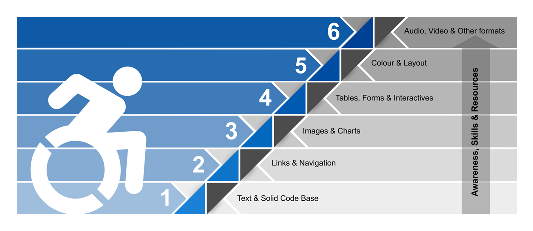
\epsfig{file=stairs-ramp.eps}
\caption{Each content type or design decision is visualized as stair or potential barrier. The numbered techniques outline how to build in the virtual ramp.}
\end{figure*}

\section{Building in the {\secit Virtual} Ramp}

\subsection{Text \& Solid Structure}

Electronic text-based content is accessible by nature. It can be rendered visually, auditorily and tactilely.

Use HTML's built-in semantic structure [1] - headings, lists, quotes - to code meaning directly into your content. 

Keep the reading level as simple as possible.

Define the natural language \& mark language changes.

Ensure there is a doctype, charset \& a unique page title in each of your templates for a valid code base.

\subsection{Navigation, Links \& Landmarks}
Navigation, links and landmarks, like stepping stones, help you find your way.

Use unique meaningful words for linked text. Keep links DRY [2] (do not repeat yourself over and over and over).

Leave context changes - pop-ups, new tabs - in the control of the user.

Use WAI-ARIA [3] landmark roles or HTML5 landmark tags to provide direct access to page content (formerly we used skip navigation links).

Design well-planned, consistent navigation. Usability helps all users.

\subsection{Images \& Charts}
Provide meaningful text alternatives for all content images. The alt attribute is required, but can be left empty, if appropriate.

For charts or complex images you may need to link to supplementary content or use the longdesc attribute.

The goal of text alternatives is to maintain the meaning of the document whether you can see the image or not.

\subsection{Tables, Forms \& Interactives}
Simplify complex HTML structures \& user interactions wherever possible.
\subsubsection{Tables}
Use the rich semantic table mark-up available in HTML - thead, tfoot, tbody. Introduce tables with the caption element. Appropriately distinguish table header cells from table data cells (th, td) on rows and columns.

Use tables only for tabular data – not content layout!

\subsubsection{Forms}
Keep forms simple – don't ask for data you don't need.

Use \& associate labels for every form control. Use the button element when you need a button.

Group form controls to create meaningful organization in forms - legend, fieldset, optgroup. Organization is good for all users.

Design clear error identification \& intuitive error handling. Clearly tell the user where they have gone wrong, how to fix the problem and when they have succeeded.

Provide reasonable time-outs (think user control).

Employ WAI-ARIA [3] standard to define roles and behaviours that HTML cannot describe. This is particularly important for interactive structures like forms.

Note: most legal cases have happened around in-accessible tables \& forms [4].

\subsection{Colour \& Layout}
Don't rely on colour alone for meaning.

Choose colours wisely \& test for sufficient contrast ratios. Avoid confusing colours. The Brewer Palette is a good resource.

Use CSS for layout  \& consistency. Using CSS \& HTML together properly is best method in making your content accessible \& easier to maintain.

\subsection{Audio, Video \& Other formats}
Do not auto-play anything (think user control).

Provide open or closed captions for audio and video.

Describe video when the meaning cannot be understood by the soundtrack alone. Video description can be open or closed.

Providing transcripts, in some cases (e.g. talking heads \& interviews), makes better sense than captions.

For other formats, such as PDF or Word documents, first ask is there a reason not to use HTML? Follow the WCAG for content in Word documents and PDFs. PDFs must be tagged to be accessible [6].

\section{Conclusions}
When web design teams ramp up a website for users of assistive technology and other edge cases, the payoff happens at many levels. The website will likely be easier to find, be of a higher quality, be easier to maintain, last longer and work better for everyone - all of which contribute to a better return on the investment. Just like accessible ramps at building entrances, the virtual ramp built into websites benefits more than the intended audience.
%\end{document}  % This is where a 'short' article might terminate

%ACKNOWLEDGMENTS are optional
\section{Acknowledgments}
Thanks to Amita Pharshy for her comments and to the {\it Accessible Icon Project} for the icon.

%REFERENCES as a SECTION
\section{References}
\begin{itemize}
\item Clark, J. (2003). {\it Building accessible websites.} Indianapolis: New Riders.
\item Clark, J. (2005). Facts and Opinions About PDF Accessibility. {\it A List Apart}. Retrieved from http://alistapart.com/article/pdf\_accessibility
\item Hanson, V. L., \& Richards, J. T. (2013). Progress on website accessibility? {\it ACM Transactions on the Web, 7}(1). DOI:10.1145/2435215.2435217
\item Horton, S. \& Quesenbery, W. (2014). {\it A Web For Everyone.} Brooklyn: Rosenfeld Media.
\item Accessible Icon Project: http://www.accessibleicon.org
\item W3C-WAI: http://www.w3.org/WAI
\item WAI-ARIA: http://www.w3.org/WAI/intro/aria.php
\item WCAG 2.0: http://www.w3.org/WAI/WCAG20/glance/Overview.html
\item WCAG Samurai: http://www.wcagsamurai.org
\item WCAG 1.0: http://www.w3.org/TR/WAI-WEBCONTENT
\item WebAIM: http://webaim.org		
\end{itemize}
%
%\section{Resources}
%\begin{itemize}
%\item Brewer Palette: http://colorbrewer2.org/
%\item HTML5: http://www.w3.org/TR/html5/
%\item W3C: http://www.w3.org/
%\item WAI: http://www.w3.org/WAI/
%\item WCAG 2.0: http://www.w3.org/WAI/WCAG20/glance/Overview.html
%\item WCAG 1.0: http://www.w3.org/TR/WAI-WEBCONTENT/
%\item WCAG Samurai: http://www.wcagsamurai.org/
%\item WAI-ARIA: http://www.w3.org/WAI/intro/aria.php
%\item Wave Accessibility Evaluation Tool: http://wave.webaim.org/
%\item WebAIM: http://webaim.org/
%\item Wikipedia: http://wikipedia.org/
%\item Paciello Group. Contrast Analyser Tool: http://www.paciellogroup.com/resources/contrastanalyser/
%\item Verou, L. Contrast Ratio Tool: http://leaverou.github.io/contrast-ratio/
%\item WebAIM Contrast Checker Tool: http://webaim.org/resources/contrastchecker/
%\end{itemize}
% The following two commands are all you need in the
% initial runs of your .tex file to
% produce the bibliography for the citations in your paper.
\bibliographystyle{abbrv}
\bibliography{sigproc}  % sigproc.bib is the name of the Bibliography in this case
% You must have a proper ".bib" file
%  and remember to run:
% latex bibtex latex latex
% to resolve all references
%
% ACM needs 'a single self-contained file'!
%
\balancecolumns
% That's all folks!
\end{document}
